\documentclass[10pt, a4paper]{scrartcl}

\usepackage{vorschule}
\usepackage[
    typ=ab,
    fach=Informatik,
    lerngruppe={Q2},
    nummer={IV.2},
    module={Symbole,Lizenzen},
    seitenzahlen=keine,
    farbig,
    lizenz=cc-by-nc-sa-4,
]{schule}

\usepackage[
	kuerzel=Ngb,
	reihe={Nichtlineare Datenstrukturen: Bäume},
	version={2020-09-16},
]{ngbschule}

\author{J. Neugebauer}
\title{Binäre Entscheidungsbäume}
\date{\Heute}

\setzeAufgabentemplate{ngbnormal}


\begin{document}

\ReiheTitel

\begin{center}
	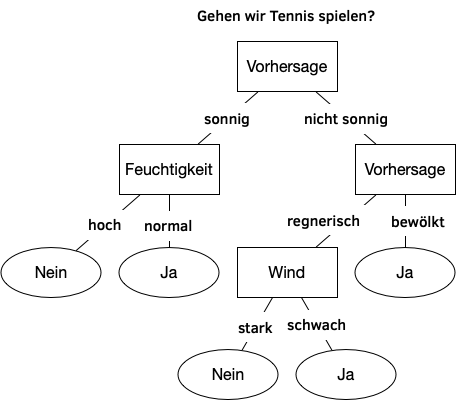
\includegraphics[width=9cm]{01-Abb_Entscheidungsbaum_Tennis.png}
\end{center}

\begin{aufgabe}
	Studiere die Dokumentation der Klasse \code{BinaryTree<ContentType>} und vergleiche sie mit der Verwendung der Klasse im Projekt \ordner{Entscheidungsbaum} im Tauschordner (in der Klasse \code{DecisionTreeBuilder}).
	
	Versuche die folgenden Leitfragen für dich zu beantworten:
	\begin{itemize}
		\item Wieso wird mehr als ein Objekt der Klasse \code{BinaryTree} erstellt?
		\item In welcher Reihenfolge wird der Baum aufgebaut (werden die Objekte der Knoten instanziiert)?
		\item Wie werden die Inhalte vom generischen Typ \code{ContentType} (hier Unterklassen der Klasse \code{Decision}) im Baum gespeichert?
	\end{itemize}
\end{aufgabe}

\begin{aufgabe}
	Die Knoten enthalten Objekte der Unterklassen von \code{Decision}. Jede Unterklasse entscheidet für einen Datensatz, ob es im Baum links oder rechts weiter geht. Die Blattknoten enthalten keine Entscheidung, sondern die finale Festlegung einer Klasse für den Datensatz (hier \enquote{Ja} oder \enquote{Nein}) in der Klasse \code{Classification}.
	
	\operator{Analysiere} die Klassen \code{Decision} und \code{Classification} und \operator{beschreibe} ihre Funktionsweise. \operator{Erkläre} auch, wie die erste Entschiedung (in der Wurzel) umgesetzt ist (Klasse \code{DecisionTreeBuilder}, Zeile 17-19). 
\end{aufgabe}

\begin{aufgabe}
	\operator{Implementiere} anhand des Beispiels im Konstruktor der Klasse \code{DecisionTreeBuilder} den vollständigen Entscheidungsbaum zur Tennis-Frage (vgl. Abbildung oben).
	
	Teste deinen Baum mit dem \emph{Objektinspektor} von \programm{BlueJ}.
\end{aufgabe}

\begin{aufgabe}
	Vervollständige die Methode \code{testeDatensatz} in \code{Entscheider}, so dass für einen Datensatz am Ende die korrekte Entscheidung (als \code{String}) zurückgegeben wird.
	
	Teste mit verschiedenen Datensätzen.
\end{aufgabe}

\end{document}
